
\begin{center}
    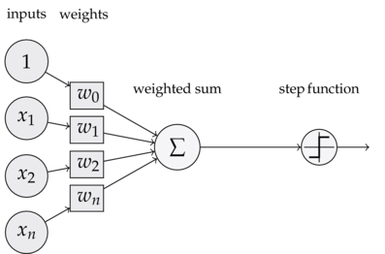
\includegraphics[width=0.6\textwidth]{Images/p_model.png} \\
\end{center}
\vspace{2mm}
Preceptron model was proposed by Frank Rosenblatt in 1943 in effort to design the model to 
mimic the human brain \citep*{939589}. Preceptron model or single layered feed forwards network 
networks takes the vectors of inputs and multiply with a randomly 
initialised weights and add random bias to network and process the information by providing data to the activation function to process the information.
There are various activation function such as  step function sigmoid, 
relu, leaky relu and other activation functions and outputs the result \citep{AGATONOVICKUSTRIN2000717}.
Figure above represents the inputs x and weights w for which weighted sum of muliplication result of 
inputs and weights will be passed to step activation function. 

\subsection*{Mathematical Representation }
\vspace{3mm}
{The equation below represents the preceptron model mentioned above in Mathematical notations.}
\begin{equation}
    \begin{split}
        y = \Big[\sigma(\sum_{k=0}^n x_k.w_k + b_k)\Big] \\
    \end{split}
\end{equation}

$ {\sigma = Activation function ,
        x = input , 
        w = weights ,
        y = prediction , 
        \sum = sum.
    } $ 
